\documentclass[aspectratio=169,11pt]{ctexbeamer}

\usetheme{Madrid}
\usecolortheme{seahorse}
\usefonttheme{professionalfonts}

\usepackage{booktabs}
\usepackage{tabularx}
\usepackage{array}
\usepackage{tikz}
\usetikzlibrary{arrows.meta,positioning,shapes.geometric,calc}

\setbeamertemplate{navigation symbols}{}
\setbeamertemplate{footline}{
  \leavevmode%
  \hbox{%
    \begin{beamercolorbox}[wd=.72\paperwidth,ht=2.4ex,dp=1ex,leftskip=1em]{author in head/foot}%
      \scriptsize Hybrid Harvesting Animal Tracker
    \end{beamercolorbox}%
    \begin{beamercolorbox}[wd=.18\paperwidth,ht=2.4ex,dp=1ex,center]{date in head/foot}%
      \scriptsize \insertshortdate
    \end{beamercolorbox}%
    \begin{beamercolorbox}[wd=.10\paperwidth,ht=2.4ex,dp=1ex,center]{date in head/foot}%
      \scriptsize \insertframenumber/\inserttotalframenumber
    \end{beamercolorbox}%
  }%
  \vskip0pt%
}
\setbeamertemplate{caption}[numbered]
\setbeamertemplate{itemize items}[circle]
\setbeameroption{hide notes}

\definecolor{HarvestBlue}{HTML}{1D4E89}
\definecolor{HarvestGreen}{HTML}{2E7D32}
\definecolor{HarvestOrange}{HTML}{F59E0B}
\definecolor{HarvestGray}{HTML}{4B5563}

\setbeamercolor{title}{fg=HarvestBlue}
\setbeamercolor{frametitle}{fg=HarvestBlue,bg=white}
\setbeamercolor{structure}{fg=HarvestBlue}
\setbeamercolor{block title}{fg=white,bg=HarvestBlue}
\setbeamercolor{block body}{fg=black,bg=blue!4}

\newcolumntype{Y}{>{\raggedright\arraybackslash}X}
\newcommand{\whday}{Wh/day}
\newcommand{\mj}{mJ}

\title[Hybrid Harvesting Animal Tracker]{Long-Term Animal Tracking System}
\subtitle{Hybrid Energy Harvesting Collar Concept}
\author[Hybrid]{Hybrid Harvesting Concept}
\institute{Micro Energy Harvesting / Uni Freiburg}
\date{\today}

\begin{document}

\begin{frame}
  \titlepage
  \note{开场：今天汇报一个面向羊体型动物的长期追踪项圈方案。重点不是单个传感器，而是怎样让系统两年内能量自给。}
\end{frame}

\begin{frame}{汇报结构}
  \begin{enumerate}
    \item 任务需求与关键约束
    \item 混合能量采集系统架构
    \item 能量预算、存储与重量估算
    \item 自适应调度与可改进方向
    \item 结论
  \end{enumerate}
  \note{给听众一个路线图：先定义问题，再证明方案能量闭合，最后讨论实际使用时如何进一步节能。}
\end{frame}

\begin{frame}{设计目标：面向羊体型动物的长期追踪}
  \begin{block}{核心任务}
    设计一个能量自给的动物追踪设备，在野外长期记录位置与活动状态。
  \end{block}

  \vspace{0.4em}
  \begin{tabularx}{\textwidth}{@{}lY@{}}
    \toprule
    需求 & 指标 \\
    \midrule
    数据频率 & 至少每 1 min 记录一次位置 + 活动数据 \\
    数据通信 & 本地存储，每几天上传到基站一次 \\
    通信范围 & 自由空间最大约 100 m \\
    使用寿命 & 至少 2 年 \\
    重量限制 & 总重量低于 1000 g \\
    工程约束 & 仅使用商业可得组件 \\
    \bottomrule
  \end{tabularx}
  \note{强调约束之间的矛盾：1分钟一次GNSS很耗能，但设备又必须轻、寿命长、野外可用。}
\end{frame}

\begin{frame}{关键挑战：GNSS 决定能耗下限}
  \begin{columns}[T,onlytextwidth]
    \begin{column}{0.52\textwidth}
      \begin{itemize}
        \item 每分钟定位一次意味着每天 1440 次 GNSS fix
        \item GNSS 与 LoRa 是主要脉冲负载，需要短时间较大电流
        \item 纯电池方案很难优雅地满足 2 年寿命
        \item 纯热电或纯动能采集功率太低，不足以支撑高频定位
      \end{itemize}
    \end{column}
    \begin{column}{0.43\textwidth}
      \begin{tikzpicture}[scale=0.9, every node/.style={font=\small}]
        \draw[fill=HarvestOrange!18,draw=HarvestOrange,rounded corners] (0,0) rectangle (4.2,3.2);
        \node[align=center,font=\bfseries] at (2.1,2.75) {能量瓶颈};
        \draw[->,very thick,HarvestOrange] (0.7,0.65) -- (0.7,2.1);
        \draw[->,very thick,HarvestOrange] (1.6,0.65) -- (1.6,1.55);
        \draw[->,very thick,HarvestOrange] (2.5,0.65) -- (2.5,1.05);
        \draw[->,very thick,HarvestOrange] (3.4,0.65) -- (3.4,0.85);
        \node[below] at (0.7,0.62) {GNSS};
        \node[below] at (1.6,0.62) {LoRa};
        \node[below] at (2.5,0.62) {MCU};
        \node[below] at (3.4,0.62) {IMU};
      \end{tikzpicture}
    \end{column}
  \end{columns}
  \note{这一页讲问题本质：不是传感器能不能买到，而是高频GNSS让能量预算很紧。}
\end{frame}

\begin{frame}{推荐方案：混合能量采集项圈}
  \begin{center}
    \begin{tikzpicture}[
      node distance=0.9cm and 1.0cm,
      box/.style={draw,rounded corners,minimum width=2.6cm,minimum height=0.85cm,align=center,font=\small},
      source/.style={box,fill=green!10,draw=HarvestGreen},
      buffer/.style={box,fill=orange!12,draw=HarvestOrange},
      load/.style={box,fill=blue!7,draw=HarvestBlue},
      arrow/.style={-{Latex[length=2.5mm]},thick}
    ]
      \node[source] (solar) {Solar panel\\主能量来源};
      \node[source,below=of solar] (kinetic) {Kinetic generator\\运动补充};
      \node[source,below=of kinetic] (thermal) {TEG module\\连续涓流};

      \node[box,right=of solar] (mppt) {Solar PMIC\\MPPT};
      \node[box,right=of kinetic] (rect) {Rectifier /\\Harvester IC};
      \node[box,right=of thermal] (boost) {Low-voltage\\boost};

      \node[buffer,right=1.1cm of rect] (storage) {Li-ion battery\\long-term buffer};
      \node[buffer,above=of storage] (cap) {LIC / Supercap\\pulse buffer};
      \node[load,right=1.1cm of storage] (loads) {MCU + GNSS\\IMU + Flash + LoRa};

      \draw[arrow] (solar) -- (mppt);
      \draw[arrow] (kinetic) -- (rect);
      \draw[arrow] (thermal) -- (boost);
      \draw[arrow] (mppt) -- (storage);
      \draw[arrow] (rect) -- (storage);
      \draw[arrow] (boost) -- (storage);
      \draw[arrow] (storage) -- (loads);
      \draw[arrow] (storage) -- (cap);
      \draw[arrow] (cap) -- (loads);
    \end{tikzpicture}
  \end{center}
  \note{核心信息：太阳能负责闭合能量预算，动能和热能增强鲁棒性，同时LIC/超级电容处理GNSS和LoRa的电流峰值。}
\end{frame}

\begin{frame}{运行假设}
  \begin{columns}[T,onlytextwidth]
    \begin{column}{0.48\textwidth}
      \begin{block}{数据采集}
        \begin{itemize}
          \item Datapoint interval: 1 min
          \item 数据内容：时间戳、GNSS 位置、睡眠/清醒状态、存储电压
          \item GNSS 仅在定位时上电
        \end{itemize}
      \end{block}
    \end{column}
    \begin{column}{0.48\textwidth}
      \begin{block}{通信与存储}
        \begin{itemize}
          \item 本地 flash 连续记录
          \item 每 3 天通过 LoRa 批量上传
          \item LoRa 与 GNSS 使用 load switch 断电
        \end{itemize}
      \end{block}
    \end{column}
  \end{columns}
  \vspace{0.6em}
  \begin{center}
    \large 目标：把高峰值功耗变成低占空比事件
  \end{center}
  \note{说明为什么用低占空比和批量上传：通信不是实时视频流，只需长期可靠记录和周期性上传。}
\end{frame}

\begin{frame}{每日能耗估算}
  \small
  \begin{tabularx}{\textwidth}{@{}lYr@{}}
    \toprule
    模块 & 假设 & 能量 \\
    \midrule
    GNSS & 621 \mj/fix，1440 fixes/day & 0.248 \whday \\
    MCU & 周期性低功耗唤醒 & 0.005 \whday \\
    Accelerometer & ADXL362，低于 2 \textmu A & 0.0002 \whday \\
    Flash logging & 每分钟写入一次 & 0.001 \whday \\
    LoRa upload & 每 3 天批量上传 & 0.006 \whday \\
    PMIC/regulator losses & 约 10--15\% 裕量 & 0.030 \whday \\
    \midrule
    \textbf{Total} & & \textbf{0.291 \whday} \\
    \bottomrule
  \end{tabularx}

  \vspace{0.8em}
  \begin{center}
    \Large \textbf{0.291 Wh/day = 1046 J/day}
  \end{center}
  \note{这里是可行性证明的第一半：负载端每天需要多少能量。指出GNSS占绝大多数，所以后续优化也主要针对GNSS。}
\end{frame}

\begin{frame}{每日采集能量估算}
  \small
  \begin{tabularx}{\textwidth}{@{}lYr@{}}
    \toprule
    来源 & 假设 & 能量 \\
    \midrule
    Solar & 2 W panel，0.5 peak sun h/day，70\% efficiency & 0.70 \whday \\
    Thermal & 100 \textmu W average & 0.0024 \whday \\
    Kinetic & 保守动物运动估计 & 0.00056 \whday \\
    \midrule
    \textbf{Total input} & & \textbf{0.703 \whday} \\
    \bottomrule
  \end{tabularx}

  \vspace{0.8em}
  \begin{columns}[T,onlytextwidth]
    \begin{column}{0.52\textwidth}
      \begin{block}{Energy margin}
        \centering
        \Large $0.703 / 0.291 \approx \textbf{2.4}$
      \end{block}
    \end{column}
    \begin{column}{0.43\textwidth}
      \small 在保守冬季太阳假设下，太阳能仍然是闭合预算的主要来源。
    \end{column}
  \end{columns}
  \note{强调热能和动能不是主供电，而是提高系统独特性和鲁棒性。真实闭合预算主要依靠小太阳能板。}
\end{frame}

\begin{frame}{能量闭合：输入大于输出}
  \begin{center}
    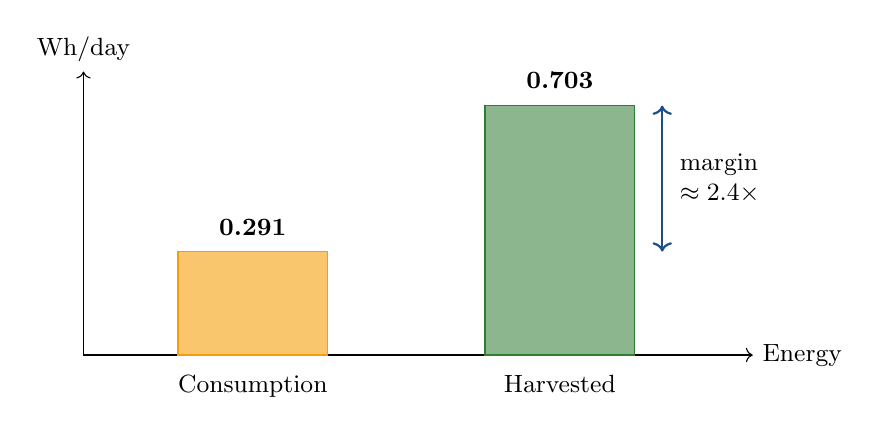
\begin{tikzpicture}[x=1cm,y=0.9cm, every node/.style={font=\small}]
      \draw[->] (0,0) -- (8.5,0) node[right]{Energy};
      \draw[->] (0,0) -- (0,4) node[above]{\whday};

      \draw[fill=HarvestOrange!60,draw=HarvestOrange] (1.2,0) rectangle (3.1,1.46);
      \node[below] at (2.15,-0.15) {Consumption};
      \node[above] at (2.15,1.55) {\textbf{0.291}};

      \draw[fill=HarvestGreen!55,draw=HarvestGreen] (5.1,0) rectangle (7.0,3.52);
      \node[below] at (6.05,-0.15) {Harvested};
      \node[above] at (6.05,3.62) {\textbf{0.703}};

      \draw[<->,thick,HarvestBlue] (7.35,1.46) -- (7.35,3.52);
      \node[right,align=left] at (7.45,2.49) {margin\\$\approx 2.4\times$};
    \end{tikzpicture}
  \end{center}
  \begin{block}{Interpretation}
    \small 在设计假设下，系统每天采集能量约为消耗的 2.4 倍，可覆盖天气、姿态和转换效率的不确定性。
  \end{block}
  \note{这是汇报中最关键的一页：用一个直观图说服听众，这个方案不是概念堆叠，而是能量上可闭合。}
\end{frame}

\begin{frame}{存储方案：长期缓冲 + 脉冲缓冲}
  \begin{columns}[T,onlytextwidth]
    \begin{column}{0.50\textwidth}
      \begin{block}{主存储}
        \centering
        1x 18650 Li-ion cell

        \vspace{0.4em}
        \Large $3.6V \times 3500mAh = 12.6Wh$
      \end{block}
      \begin{block}{无采集续航}
        \centering
        \Large $12.6 / 0.291 \approx 43$ days
      \end{block}
    \end{column}
    \begin{column}{0.46\textwidth}
      \begin{block}{脉冲缓冲}
        \begin{itemize}
          \item 30 F LIC 或 supercapacitor
          \item 缓冲 GNSS 与 LoRa 峰值电流
          \item 减少电池瞬态负担
          \item 改善低温或老化情况下的稳定性
        \end{itemize}
      \end{block}
    \end{column}
  \end{columns}
  \note{解释为什么同时需要电池和超级电容：电池提供天级能量，电容提供秒级功率。}
\end{frame}

\begin{frame}{组件候选}
  \small
  \begin{tabularx}{\textwidth}{@{}lY@{}}
    \toprule
    功能 & 候选组件 \\
    \midrule
    Solar harvester & Voltaic Systems 2 W / 6 V flexible panel \\
    Kinetic harvester & Kinetron MSG32 / mechanical generator system \\
    Thermal harvester & TEC Microsystems 1MC06-048-15\_TEG 或 Matrix thermal module \\
    Solar PMIC & e-peas AEM10941 \\
    Thermal PMIC & Matrix MCRY12, LTC3108, AEM20940 \\
    GNSS & u-blox MAX-M10S \\
    Activity sensor & Analog Devices ADXL362 \\
    MCU & TI MSP430FR5969 或 STM32L4 \\
    Wireless & Semtech SX1262 LoRa \\
    Memory / switch & SPI NOR flash, Vishay SIP32431 \\
    \bottomrule
  \end{tabularx}
  \note{这一页快速扫过即可，重点是说明所有部件都是商业可得，不依赖实验室自制器件。}
\end{frame}

\begin{frame}{重量估算}
  \small
  \begin{tabularx}{0.86\textwidth}{@{}lr@{}}
    \toprule
    部件 & 重量 \\
    \midrule
    2 W solar panel & 60--100 g \\
    Kinetic generator & 18--30 g \\
    Thermal modules + heat spreader & 60--100 g \\
    18650 battery & 45--50 g \\
    LIC / supercap & 20--40 g \\
    PCB + electronics + antenna & 30--60 g \\
    Enclosure & 100--200 g \\
    Collar / mounting & 150--250 g \\
    \midrule
    \textbf{Total estimate} & \textbf{500--830 g} \\
    \bottomrule
  \end{tabularx}

  \vspace{0.5em}
  \begin{center}
    \Large 低于 1000 g 限制，并保留机械设计余量
  \end{center}
  \note{说明重量不是瓶颈，但机械封装、动物舒适性和防水仍然需要后续工程验证。}
\end{frame}

\begin{frame}{改进方向 1：动能采集器兼作活动指示器}
  \begin{columns}[T,onlytextwidth]
    \begin{column}{0.48\textwidth}
      \begin{itemize}
        \item 每分钟 pulse count
        \item 峰值电压
        \item 每分钟采集能量
        \item 超过阈值的时间
      \end{itemize}
    \end{column}
    \begin{column}{0.48\textwidth}
      \small
      \begin{tabularx}{\textwidth}{@{}lY@{}}
        \toprule
        Kinetic signal & Activity \\
        \midrule
        almost no pulses & sleeping / resting \\
        low intermittent pulses & awake / grazing \\
        frequent high pulses & walking / running \\
        \bottomrule
      \end{tabularx}
    \end{column}
  \end{columns}
  \vspace{0.8em}
  \begin{block}{定位}
    加速度计仍是主要活动传感器；动能信号可作为被动、低成本的辅助活动特征。
  \end{block}
  \note{这页体现方案的动物特异性：运动不仅是能量来源，也能贡献行为信息。}
\end{frame}

\begin{frame}{改进方向 2：自适应 GNSS 间隔}
  \small
  \begin{tabularx}{\textwidth}{@{}lY@{}}
    \toprule
    状态 & GNSS strategy \\
    \midrule
    sleeping / resting & 重用上次位置，或每 10--30 min 定位一次 \\
    grazing / slow movement & 每 5 min 定位一次 \\
    active / walking & 每 1 min 定位一次 \\
    low storage voltage & 降低 GNSS 频率，优先保存活动日志 \\
    \bottomrule
  \end{tabularx}

  \vspace{0.8em}
  \begin{center}
    \Large 关键思想：位置数据频率随信息价值变化
  \end{center}
  \note{讲清楚：不是所有状态都需要同样的定位频率。休息时高频GNSS信息价值低，节能潜力大。}
\end{frame}

\begin{frame}{改进方向 3：Energy-Aware Scheduler}
  \begin{center}
    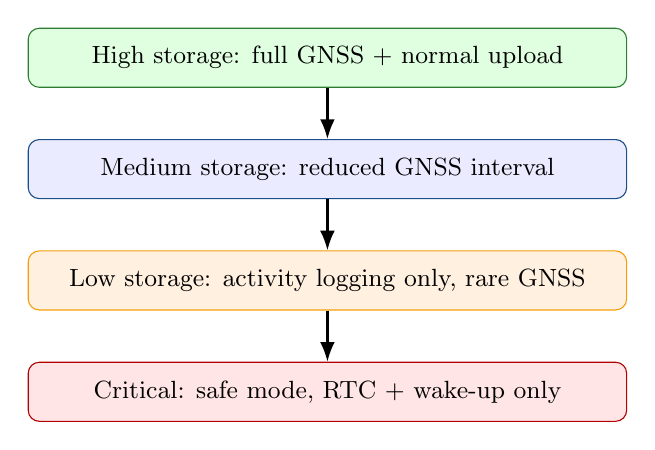
\begin{tikzpicture}[
      node distance=0.65cm,
      state/.style={draw,rounded corners,minimum width=7.6cm,minimum height=0.75cm,align=center,font=\small},
      arrow/.style={-{Latex[length=2.5mm]},thick}
    ]
      \node[state,fill=green!12,draw=HarvestGreen] (high) {High storage: full GNSS + normal upload};
      \node[state,fill=blue!8,draw=HarvestBlue,below=of high] (medium) {Medium storage: reduced GNSS interval};
      \node[state,fill=orange!12,draw=HarvestOrange,below=of medium] (low) {Low storage: activity logging only, rare GNSS};
      \node[state,fill=red!10,draw=red!70!black,below=of low] (critical) {Critical: safe mode, RTC + wake-up only};
      \draw[arrow] (high) -- (medium);
      \draw[arrow] (medium) -- (low);
      \draw[arrow] (low) -- (critical);
    \end{tikzpicture}
  \end{center}
  \note{解释调度器像一个能量管理策略：根据电池电压选择服务质量，确保系统不会完全掉电。}
\end{frame}

\begin{frame}{风险与验证计划}
  \begin{columns}[T,onlytextwidth]
    \begin{column}{0.48\textwidth}
      \begin{block}{主要风险}
        \begin{itemize}
          \item 太阳能板被毛发、泥土或姿态遮挡
          \item 热电温差可能低于预期
          \item 动能采集与动物舒适性冲突
          \item 野外 LoRa 链路受地形影响
        \end{itemize}
      \end{block}
    \end{column}
    \begin{column}{0.48\textwidth}
      \begin{block}{验证步骤}
        \begin{itemize}
          \item 桌面功耗测量：GNSS / LoRa / sleep
          \item 日照与姿态采样测试
          \item 运动台或实地动能采集测试
          \item 100 m LoRa 链路测试
        \end{itemize}
      \end{block}
    \end{column}
  \end{columns}
  \note{这一页让方案更可信：承认可变因素，并给出可执行的验证计划。}
\end{frame}

\begin{frame}{关键结论}
  \begin{block}{结论 1}
    纯热电 + 纯动能不足以支持每分钟一次 GNSS 定位。
  \end{block}
  \begin{block}{结论 2}
    小型太阳能板 + 动能采集 + 热电涓流 + 可充电存储，是更稳健的混合方案。
  \end{block}
  \begin{block}{结论 3}
    估算结果显示：每日消耗 0.291 \whday，每日采集 0.703 \whday，能量裕量约 2.4，总重量约 500--830 g。
  \end{block}
  \note{收束：方案在能量、重量和组件可得性上都满足需求，后续重点转向实测与调度策略优化。}
\end{frame}

\begin{frame}
  \centering
  \Huge Thank you

  \vspace{1em}
  \Large Questions?
  \note{结束页。可以准备回答：为什么不用蜂窝网络、为什么不是太阳能单独方案、冬季/遮挡怎么办。}
\end{frame}

\end{document}
